\documentclass[11pt,a4paper]{article}

% ── Core packages — all available in Overleaf ─────────────────────────────────
\usepackage[utf8]{inputenc}
\usepackage[T1]{fontenc}
\usepackage{microtype}
\usepackage[margin=1in]{geometry}
\usepackage{amsmath,amssymb,amsfonts,amsthm}
\usepackage{graphicx}
\usepackage{booktabs}
\usepackage{multirow}
\usepackage{subcaption}
\usepackage{float}
\usepackage{xcolor}
\usepackage{algorithm}
\usepackage{algpseudocode}
\usepackage[round,sort]{natbib}
\usepackage{hyperref}
\usepackage{url}
\usepackage{enumitem}
\usepackage{tabularx}
\usepackage{array}
\usepackage{setspace}

% ── Hyperref configuration ────────────────────────────────────────────────────
\hypersetup{
    colorlinks = true,
    linkcolor  = blue!70!black,
    citecolor  = green!50!black,
    urlcolor   = blue!80!black,
    pdftitle   = {Invisible Bridges},
    pdfauthor  = {Amit Kumar}
}

% ── Custom maths commands ─────────────────────────────────────────────────────
\newcommand{\bscore}{C(u;\mathcal{P})}
\newcommand{\amp}{A(u;\mathcal{P})}
\newcommand{\R}{\mathbb{R}}
\newcommand{\E}{\mathbb{E}}
\newcommand{\hb}{\bar{h}}

\theoremstyle{definition}
\newtheorem{definition}{Definition}[section]
\theoremstyle{plain}
\newtheorem{proposition}{Proposition}[section]

% ── Title block ───────────────────────────────────────────────────────────────
\title{%
    \LARGE\textbf{Invisible Bridges:}\\[4pt]
    \Large A Downstream Sensitivity Metric Identifies\\
    Causally Critical Attention Heads\\
    Missed by Magnitude-Based Pruning%
}

\author{%
    Amit Kumar\\[2pt]
    \small\textit{Independent Researcher}\\
    \small\texttt{[contact email]}%
}

\date{\today}

% ═════════════════════════════════════════════════════════════════════════════
\begin{document}

\maketitle
\thispagestyle{empty}

% ── Abstract ─────────────────────────────────────────────────────────────────
\begin{abstract}
\noindent
We identify a class of attention heads in transformer language models that
are systematically overlooked by magnitude-based pruning metrics yet cause
catastrophic performance degradation when removed.
We call these \emph{invisible bridges} and show they are detectable by a
purely observational metric, \emph{downstream representation
sensitivity}, computed without fine-tuning or gradient access.
%
In GPT-2 Small, three Layer-0 heads with near-minimum weight magnitude
produce 21--272\% perplexity increases when ablated, compared with 0.4\%
for weight-matched controls (damage ratio: $213\times$).
%
Layer-0 position is insufficient to explain this: low-bridge Layer-0 controls cause
only 2.7\% damage.
Attention-sink behaviour is insufficient to explain it: bridge heads
exhibit high attention variance across diverse inputs ($\sigma > 0.09$),
inconsistent with rigid position-0 routing.
%
The metric predicts causal importance \emph{prospectively}: a head
identified solely by bridge score occupies the correct ordinal position
on the damage spectrum before any ablation is conducted;
the same ordinal prediction holds for independently discovered candidates
in GPT-2 Medium.
%
Mechanistic analysis shows that downstream perturbation amplification
tracks bridge score in GPT-2 Small ($r=+0.875$, $n=12$,
$p<0.001$; 95\% bootstrap CI $[0.80,\, 0.98]$) and
GPT-2 Medium ($r=+0.715$, $n=16$, $p<0.002$;
95\% bootstrap CI $[0.40,\, 0.90]$), supporting the interpretation that
bridge score preferentially identifies attention heads whose perturbations
are associated with greater downstream amplification rather than absorption.
These findings challenge a core assumption of neural-network pruning:
for the most structurally critical heads, weight magnitude and causal
importance are not merely uncorrelated---their rankings are inverted.
\end{abstract}

\newpage
\setcounter{page}{1}
\tableofcontents
\vspace{1em}

% ═════════════════════════════════════════════════════════════════════════════
\section{Introduction}
\label{sec:intro}

Every magnitude-based pruning method rests on the same implicit bet:
that a weight's size is a reliable proxy for its functional importance.
Small weights are removed; large weights are retained.
This assumption is practically appealing---magnitude is cheap to compute,
gradient-free, and scales trivially to billion-parameter models---and
underlies a decade of successful work from early weight pruning
\citep{han2015learning} through lottery tickets \citep{frankle2019lottery}
to modern one-shot methods such as SparseGPT \citep{frantar2023sparsegpt}
and Wanda \citep{sun2024wanda}.

But what if the bet is wrong precisely where it matters most?

We present empirical evidence that it is.
In GPT-2 Small \citep{radford2019gpt2}, we identify a class of attention
heads that possess near-minimum weight magnitude by every standard metric,
including the state-of-the-art Wanda criterion, yet are \emph{causally
essential} to model performance.
Ablating three such heads individually produces 21--272\% perplexity
increases; ablating weight-matched controls produces $<1\%$.
The mean damage ratio is $213\times$.
The heads that magnitude-based methods would prune first are, for this
class, the heads that matter most.

These heads are not attention sinks \citep{xiao2024sinks}: their
attention distributions vary substantially across inputs
($\sigma > 0.09$).
Their criticality is not explained by layer position: low-bridge Layer-0
controls cause near-zero damage.
Their importance is not detected by Wanda: the two metrics are nearly
orthogonal (Pearson $r \approx 0$ across all domains).

We term these heads \emph{invisible bridges}, drawing on the notion of
bridge nodes in graph percolation theory
\citep{broadbent1957percolation,freeman1977betweenness}: low-weight
connectors whose removal disconnects load-bearing paths in a network.
The analogy extends to Lagrangian coherent structures in turbulent flows
\citep{haller2000lagrangian}: locally unremarkable material lines whose
disruption collapses global transport structure.
Invisible bridge heads play an analogous role: locally unremarkable
by weight magnitude, yet their ablation collapses downstream
representation structure in a way that nothing in the network
compensates for.

\paragraph{Contributions.}
\begin{enumerate}[leftmargin=*,topsep=2pt,itemsep=2pt]
    \item We define \emph{downstream representation sensitivity}
    $C(u;\mathcal{P})$, a gradient-free, probe-based metric that measures
    how much ablating a head shifts the representations of all subsequent
    layers (Section~\ref{sec:method}).
    \item We show $C(u;\mathcal{P})$ is nearly orthogonal to Wanda
    ($r\approx 0$) and identifies heads with up to $213\times$ more causal
    damage than weight-matched controls (Section~\ref{sec:causal}).
    \item We demonstrate that $C(u;\mathcal{P})$ predicts the causal
    importance of previously unseen heads \emph{prospectively}, within
    GPT-2 Small and independently in GPT-2 Medium
    (Section~\ref{sec:prediction}).
    \item We show that downstream perturbation amplification
    correlates with bridge score in both models ($r=+0.875$, $r=+0.715$),
    providing mechanistic evidence
    (Section~\ref{sec:mechanism}).
    \item We introduce domain-conditional bridge scores
    ($C_{\text{code}},\, C_{\text{math}},\, C_{\text{lang}}$) that expose
    functional specialisation compressed by scalar aggregation
    (Section~\ref{sec:domain_results}).
\end{enumerate}

% ═════════════════════════════════════════════════════════════════════════════
\section{Related Work}
\label{sec:related}

\subsection{Magnitude-Based and Data-Free Pruning}

\citet{han2015learning} established magnitude-based weight pruning for deep
networks.
\citet{frankle2019lottery} showed that dense networks contain sparse
subnetworks (``winning tickets'') that can be retrained in isolation, though
identifying them requires a full training run.
SparseGPT \citep{frantar2023sparsegpt} and Wanda \citep{sun2024wanda}
extend one-shot pruning to large language models without retraining; Wanda
uses the product of weight magnitude and input activation norm and
currently represents the state of the art in cheap, gradient-free pruning.
Data-free methods including Synflow \citep{tanaka2020synflow} and GraSP
\citep{wang2020grasp} avoid training-data dependency; RigL
\citep{evci2020rigging} learns sparse structure during training.
None of these methods account for the relational, structural-graph
importance that our metric captures.

\subsection{Attention Head Analysis}

\citet{michel2019sixteen} showed that many attention heads can be pruned
without measurable loss on downstream benchmarks.
\citet{voita2019analyzing} identified specialised head functions whose
removal degrades performance more than random ablation.
LLM-Pruner \citep{ma2023llmpruner} extends structured pruning to
coupled components in large models.
Our contribution differs: we identify heads that are functionally critical
\emph{despite} appearing unimportant by every magnitude-based criterion
currently in use.

\subsection{Mechanistic Interpretability}

\citet{elhage2021mathematical} introduced the circuits framework for
understanding transformer computation via residual stream decomposition.
\citet{olsson2022induction} characterised induction heads as functionally
important two-layer circuits identifiable through activation patching.
\citet{conmy2023acdc} automated circuit discovery via causal interventions.
\citet{meng2022rome} localised factual associations in GPT through a
causal mediation analysis of the residual stream.
Our work is complementary: rather than identifying specific algorithms, we
discover heads whose ablations produce growing downstream disruption-a
dynamical property not previously characterised in the circuits literature.
Centred kernel alignment \citep{kornblith2019cka} provides a related
framework for measuring representational similarity across layers.

\subsection{Attention Sinks}

\citet{xiao2024sinks} showed that certain heads consistently route excess
probability mass to a fixed position-0 token, appearing important by
attention-weight inspection but structurally benign.
We explicitly test for and rule out attention-sink behaviour as an
alternative explanation for bridge criticality through attention variance
analysis (Section~\ref{sec:confounds}).

\subsection{Structural Importance in Networks and Physics}

The observation that low-weight connectors can be structurally critical
has deep roots outside machine learning.
In percolation theory, \citet{broadbent1957percolation} showed that global
network connectivity is controlled by a small number of edges near a
critical threshold, not by mean edge weight.
\citet{freeman1977betweenness} formalised betweenness centrality as a
measure of a node's indispensability to information flow; bridge nodes have
high betweenness independent of their degree.
In fluid dynamics, \citet{hunt1988eddies} introduced the Q-criterion for
identifying coherent vortical structures in turbulent flow that organise
global transport despite being locally unremarkable by velocity magnitude.
\citet{haller2000lagrangian} extended this framework to Lagrangian
coherent structures: material surfaces that act as invisible transport
barriers, separating regions of qualitatively different dynamics.
These concepts motivate our intuition that structural importance in a
computational graph need not correlate with component size.

% ═════════════════════════════════════════════════════════════════════════════
\section{Downstream Representation Sensitivity}
\label{sec:method}

\subsection{Motivation}
\label{sec:motivation}

Standard pruning importance scores are \emph{local}: they assign a value
to each weight as a function of that weight and its immediate input.
Wanda's per-head score,
\begin{equation}
    W(u) \;=\;
    \bigl\|X_{[s:e]}\bigr\|_{F}
    \cdot
    \bigl\|W_{[s:e,:]}\bigr\|_{1},
    \label{eq:wanda}
\end{equation}
measures how much the weight magnifies its input, but not what downstream
computations depend on that output.

A head may have small weight magnitude because it is doing
\emph{precision routing}, selectively forwarding a specific signal whose
content is used by many subsequent layers.
If downstream layers build their representations on top of that signal,
removing it causes cascading disruption.
The local score is blind to this cascade; our metric is not.

\subsection{Metric Definition}
\label{sec:definition}

Let $M$ be a transformer with $L$ layers and $H$ attention heads per layer.
Let $\hb_l(x) \in \R^{d}$ denote the residual-stream hidden state at
layer $l$ for input $x$, mean-pooled over the sequence dimension.
For unit $u = (l_u, k)$ (layer $l_u$, head index $k$), let
$\hb_l^{(u)}(x)$ denote the same quantity after ablating~$u$.

\begin{definition}[Downstream Representation Sensitivity]
\label{def:bridge}
\begin{equation}
    C(u;\mathcal{P}) \;=\;
    \E_{x \sim \mathcal{P}}\!\left[
        \frac{1}{L - l_u - 1}
        \sum_{l=l_u+1}^{L}
        \bigl\| \hb_l(x) - \hb_l^{(u)}(x) \bigr\|_2
    \right].
    \label{eq:bridge}
\end{equation}
\end{definition}

Intuitively, $C(u;\mathcal{P})$ measures how much ablating $u$ shifts all
downstream residual-stream representations on average.
A head that is irrelevant to downstream computation produces
$C(u;\mathcal{P}) \approx 0$; a head whose output is used by many
subsequent layers produces large $C$.

\paragraph{Ablation mechanism.}
For head $u=(l_u,k)$ with $d_h = d/H$, we zero the slice
$[s\!:\!e] = [k d_h\!:\!(k\!+\!1)d_h]$ in the input to
$c_{\text{proj}}$ at layer $l_u$ via a PyTorch
\texttt{register\_forward\_pre\_hook}.
This prevents head~$k$'s attention output from contributing to the
projected residual update while leaving all other heads intact.
The result is mathematically equivalent to zeroing the corresponding rows
of the $c_{\text{proj}}$ weight matrix.

\subsection{Downstream Amplification}
\label{sec:amp_def}

To characterise the dynamical profile of a head's perturbation we define:
\begin{equation}
    A(u;\mathcal{P}) \;=\;
    \E_{x \sim \mathcal{P}}\!\bigl[
        \delta_L(u,x) - \delta_1(u,x)
    \bigr],
    \label{eq:amp}
\end{equation}
where $\delta_l(u,x) = \|\hb_l(x) - \hb_l^{(u)}(x)\|_2$.
$A(u) > 0$ indicates that the perturbation grows toward the output layers
(amplification); $A(u) < 0$ indicates rapid absorption.

\subsection{Domain-Conditional Scores}
\label{sec:domain_def}

The scalar $C(u;\mathcal{P})$ aggregates over a mixed probe set, compressing
domain-specific structure.
We define domain-conditional scores $C_d(u) = C(u;\mathcal{P}_d)$ for
$d \in \{\text{code, math, lang}\}$, where $\mathcal{P}_d$ consists solely
of domain-$d$ texts.
The specialisation gap $\Delta(u) = \max_d C_d(u) - C(u;\mathcal{P}_{\text{mix}})$
measures how much the scalar underestimates the head's peak importance.

\subsection{Algorithm and Computational Cost}

\begin{algorithm}[t]
\caption{Compute $C(u;\mathcal{P})$ for all heads at layer $l_u$}
\label{alg:bridge}
\begin{algorithmic}[1]
\Require{Model $M$, probe texts $\mathcal{P}$, target layer $l_u$}
\Ensure{Scores $C[k]$ for $k \in \{0,\ldots,H-1\}$}
\ForAll{$x \in \mathcal{P}$}
    \State Run $M(x)$; record $\hb_l(x)$ for all $l > l_u$ \Comment{Baseline}
\EndFor
\For{$k \gets 0$ \textbf{to} $H-1$}
    \State $s \gets k \cdot d_h$;\quad $e \gets (k+1)\cdot d_h$
    \State Register pre-hook on $c_{\text{proj}}[l_u]$: zero input slice $[s:e]$
    \ForAll{$x \in \mathcal{P}$}
        \State Run $M(x)$; record $\hb_l^{(k)}(x)$ for all $l > l_u$
    \EndFor
    \State Remove hook
    \State $C[k] \gets \frac{1}{|\mathcal{P}|(L-l_u-1)}
              \displaystyle\sum_{x,l}\bigl\|\hb_l(x)-\hb_l^{(k)}(x)\bigr\|_2$
\EndFor
\State \Return{$C$}
\end{algorithmic}
\end{algorithm}

Algorithm~\ref{alg:bridge} requires $2H|\mathcal{P}|$ forward passes (one
baseline set, one per head per probe).
No backward passes or gradient storage are needed.
With $|\mathcal{P}|=15$ probe texts and $H=12$ heads, the full scan
completes in under 3 minutes on a consumer GPU (NVIDIA RTX series).
The same code runs unchanged on GPT-2 Small and GPT-2 Medium.

% ═════════════════════════════════════════════════════════════════════════════
\section{Experimental Setup}
\label{sec:setup}

\paragraph{Models.}
\textbf{GPT-2 Small}: 117M parameters, 12 layers, 12 heads/layer,
$d=768$ \citep{radford2019gpt2}.
\textbf{GPT-2 Medium}: 345M parameters, 24 layers, 16 heads/layer,
$d=1024$.
All experiments use frozen, locally-cached weights.

\paragraph{Probe set.}
$|\mathcal{P}|=15$ texts per domain: 5 code snippets (Python/SQL),
5 mathematical paragraphs (calculus, linear algebra, probability), 5
natural language passages (narrative, expository, journalistic).
The probe set is fixed before any ablation experiment.

\paragraph{Evaluation corpus.}
A disjoint 24-text held-out corpus (8 per domain) is used for all
perplexity measurements.

\paragraph{Baseline importance metric.}
The head-level Wanda score aggregates Equation~\eqref{eq:wanda} over all
weights in the $c_{\text{proj}}$ slice for head $u$.

\paragraph{Ablation.}
All ablations zero the $c_{\text{proj}}$ input slice for the target head
and measure perplexity on the full 24-text evaluation corpus using
\texttt{GPT2LMHeadModel}.

\paragraph{Experimental phases.}
Results are presented in five successive phases, each adding an independent
layer of evidence:
(0)~metric independence,
(1)~causal validation,
(1.5)~confound elimination,
(2)~prospective prediction,
(3/4)~mechanistic analysis.

% ═════════════════════════════════════════════════════════════════════════════
\section{Results}
\label{sec:results}

\subsection{Phase 0: Metric Independence}
\label{sec:discovery}

\begin{figure}[t]
    \centering
    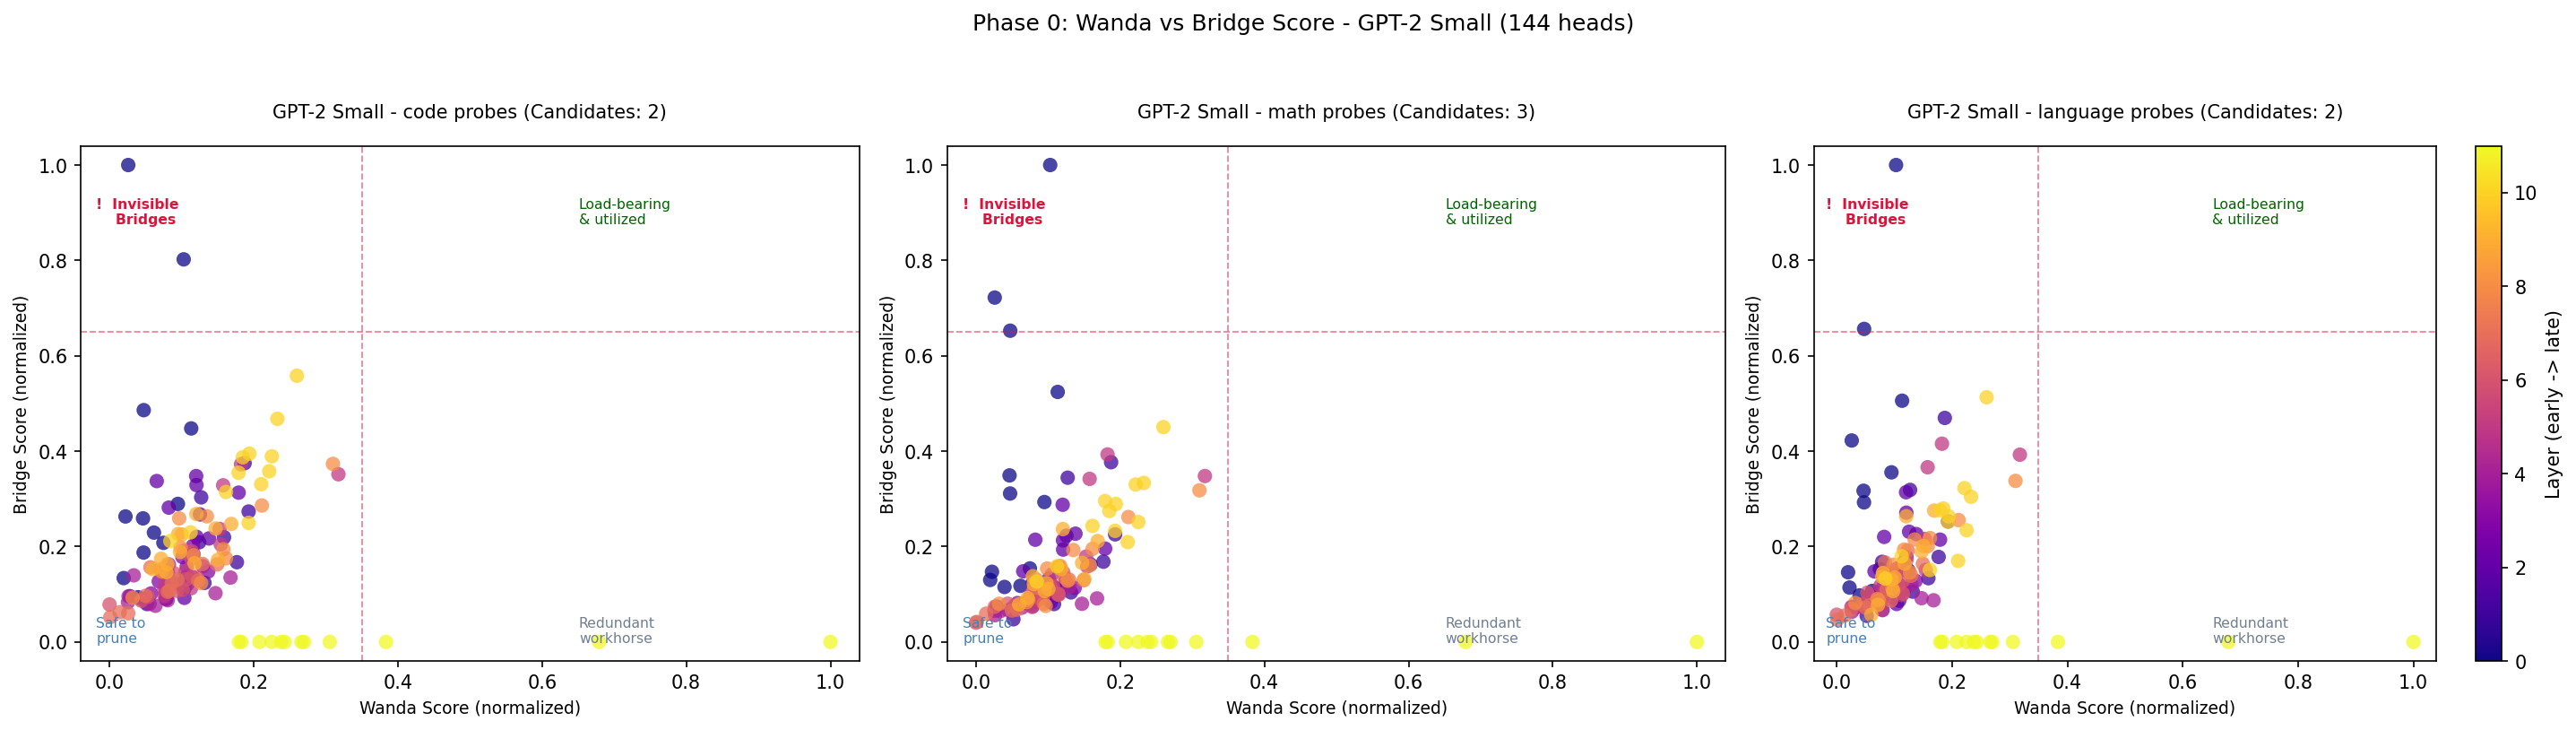
\includegraphics[width=\linewidth]{phase0_scatter.png}
    \caption{%
        \textbf{Bridge score vs.\ Wanda score (GPT-2 Small, 144 heads).}
        Each point is a Layer-0 attention head, coloured by layer depth
        (early: dark; late: bright).
        Pearson $r \in [-0.054, -0.027]$ across probe domains, the two
        metrics are nearly orthogonal and slightly anti-correlated.
        Three heads form a distinct population in the top-left
        (\emph{invisible bridge}) quadrant: L00H00, L00H07, L00H10.
    \label{fig:scatter}}
\end{figure}

Figure~\ref{fig:scatter} shows the joint distribution of $C(u)$ and $W(u)$
for all 144 heads of GPT-2 Small.
Across all probe domains, the Pearson correlation between bridge score and
Wanda score satisfies $r \in [-0.054, -0.027]$: the metrics are nearly
orthogonal.
The slight negative correlation is noteworthy: heads with the highest Wanda
scores are marginally \emph{less} likely to have high bridge scores,
suggesting that high-weight-magnitude heads are somewhat more redundant,
with alternative paths compensating for their removal.

Three heads form a clear population in the invisible bridge quadrant
(normalised Wanda $< 0.35$, normalised bridge $> 0.65$):
\begin{itemize}[topsep=2pt,itemsep=1pt]
    \item L00H00: $W_{\text{norm}}=0.026$, $C_{\text{norm}}=1.00$
    \item L00H07: $W_{\text{norm}}=0.047$, $C_{\text{norm}} \approx 0.65$--$0.80$
    \item L00H10: $W_{\text{norm}}=0.103$, $C_{\text{norm}} \approx 0.80$--$1.00$
\end{itemize}

\subsection{Phase 1: Causal Validation}
\label{sec:causal}

\begin{table}[t]
\centering
\caption{%
    \textbf{Phase 1 ablation results (GPT-2 Small).}
    Groups:
    \textbf{A} invisible bridge candidates;
    \textbf{B} Wanda-matched controls (Layers 4--7);
    \textbf{C} top-3 heads by Wanda score;
    \textbf{D} all three bridge heads ablated simultaneously.
    Baseline perplexities: code 23.45, math 58.35, language 22.62.
\label{tab:phase1}}
\small
\setlength{\tabcolsep}{5pt}
\begin{tabular}{llrrr}
\toprule
\textbf{Group} & \textbf{Head} &
\textbf{Code $\Delta\%$} & \textbf{Math $\Delta\%$} & \textbf{Lang.\ $\Delta\%$} \\
\midrule
\multirow{3}{*}{A (Bridges)}
  & L00H00 & $+158.1$ & $+21.6$  & $+24.6$ \\
  & L00H07 & $+30.4$  & $+84.1$  & $+31.9$ \\
  & L00H10 & $+106.9$ & $+152.8$ & $+272.3$ \\
\addlinespace
\multirow{3}{*}{B (Wanda ctrl.)}
  & L07H07 & $+1.2$  & $+1.9$  & $-0.2$ \\
  & L04H05 & $+0.7$  & $+0.3$  & $+0.3$ \\
  & L07H00 & $-0.8$  & $-0.4$  & $+0.5$ \\
\addlinespace
\multirow{3}{*}{C (High-Wanda)}
  & L11H00 & $+13.3$ & $+6.3$  & $+10.4$ \\
  & L11H08 & $+5.0$  & $+5.5$  & $+7.7$  \\
  & L11H11 & $+2.6$  & $+0.2$  & $+0.4$  \\
\addlinespace
D (All bridges) & ---
  & $+139.3$ & $+217.3$ & $+207.1$ \\
\midrule
\multicolumn{2}{l}{\textbf{Mean damage ratio A\,/\,B}}
  & \multicolumn{3}{c}{$\mathbf{213\times}$} \\
\bottomrule
\end{tabular}
\end{table}

Table~\ref{tab:phase1} reports perplexity damage for all ablation groups.
The mean damage ratio between Group~A and the Wanda-matched controls
(Group~B) is $213\times$.
Crucially, the high-Wanda heads (Group~C) cause only 5--13\% damage
despite being ranked most important by magnitude metrics, while the three
invisible bridge heads cause 22--272\%.
The Wanda importance ranking is \emph{inverted} for the most structurally
critical parameters in the model.

Each bridge head exhibits a distinct \emph{domain fingerprint}:
L00H00 is code-dominant ($+158\%$ code vs.\ $+22\%$ math);
L00H07 is math-dominant ($+84\%$ math vs.\ $+30\%$ code);
L00H10 causes severe damage across all three domains.

\subsection{Phase 1.5: Confound Elimination}
\label{sec:confounds}

\begin{figure}[t]
    \centering
    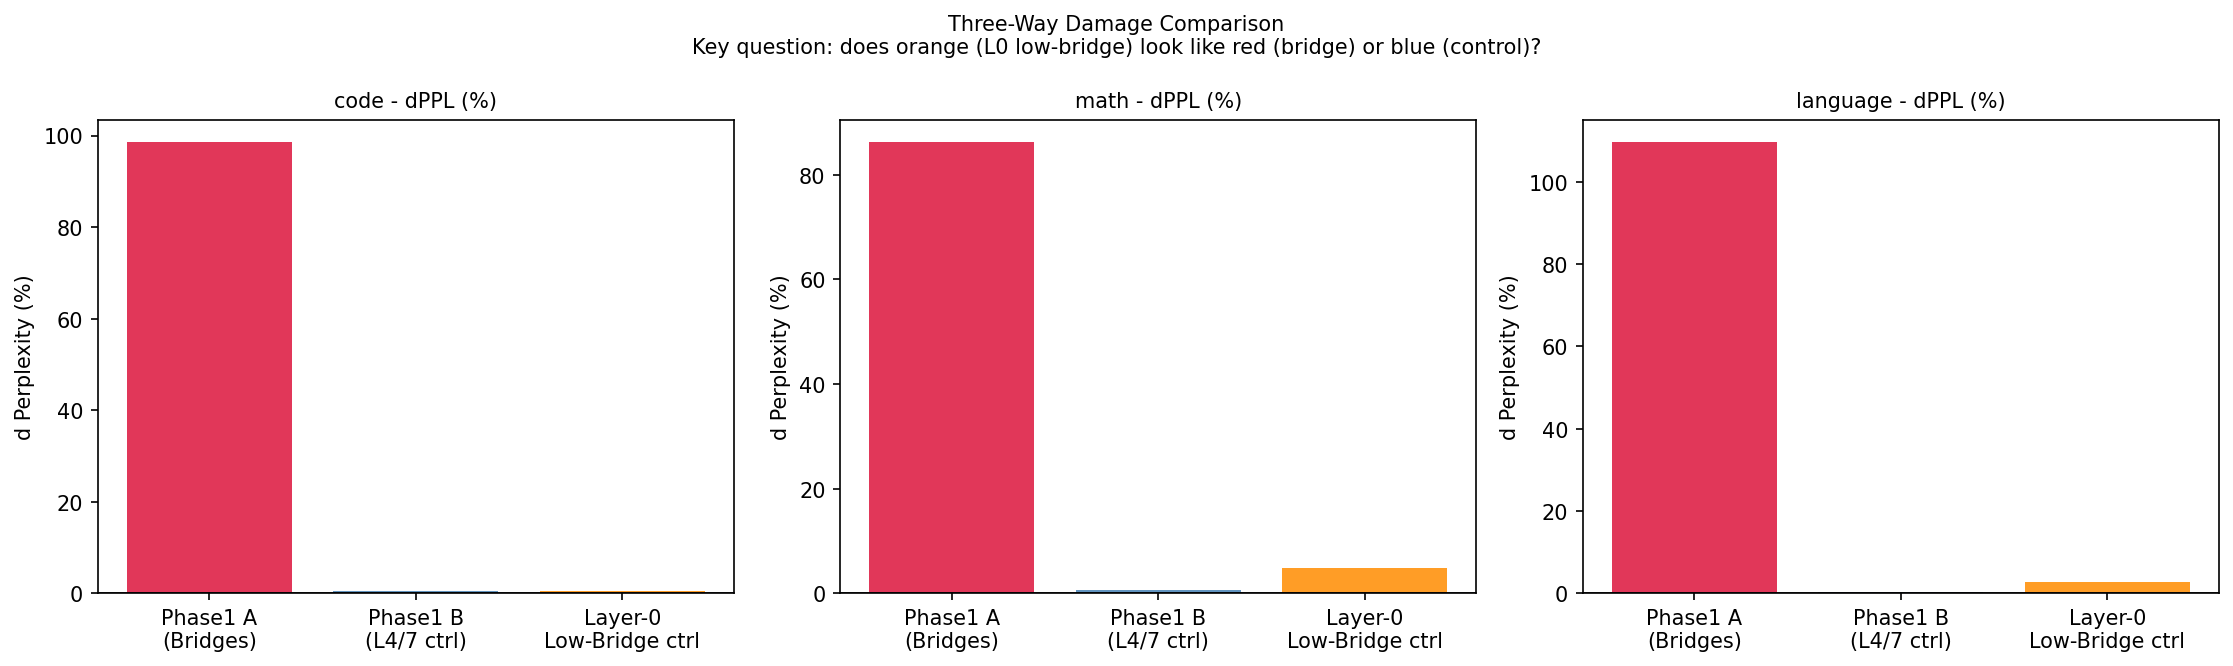
\includegraphics[width=\linewidth]{phase1_5_comparison.png}
    \caption{%
        \textbf{Three-way damage comparison (GPT-2 Small).}
        Red: bridge candidates ($\approx 98$--$110\%$).
        Blue: Wanda-matched Layer-4/7 controls ($< 1\%$).
        Orange: low-bridge Layer-0 controls ($2.7\%$).
        Orange is indistinguishable from blue, ruling out Layer-0 position
        as an explanation for bridge-head criticality.
    \label{fig:threeway}}
\end{figure}

\paragraph{Layer-0 position.}
All three bridge candidates reside in Layer~0.
The alternative hypothesis is that any Layer-0 head has elevated importance
regardless of bridge score.
We test this by ablating the three lowest-bridge Layer-0 heads
(L00H04: $C=2.88$; L00H11: $C=4.11$; L00H08: $C=5.73$).
Mean perplexity damage: $2.7\%$ (Figure~\ref{fig:threeway}).
This is indistinguishable from the Layer-4/7 controls ($<1\%$) and
$35\times$ below the bridge candidates ($\approx 98\%$).
Layer-0 position alone does not account for bridge criticality.
The same pattern holds in GPT-2 Medium, where low-bridge Layer-0 heads
cause $0$--$7\%$ damage.

\paragraph{Attention-sink behaviour.}
\begin{table}[t]
\centering
\caption{%
    \textbf{Attention-sink variance test.}
    Mean and standard deviation of attention assigned to position~0
    across 12 diverse probe texts.
    True sinks exhibit $\sigma \approx 0$.
    All three bridge heads show substantial variance, inconsistent with
    rigid BOS-token routing.
\label{tab:sinks}}
\small
\begin{tabular}{lrrll}
\toprule
\textbf{Head} & \textbf{Mean} & \textbf{Std} & \textbf{Range} &
\textbf{Verdict} \\
\midrule
L00H00 & 0.394 & 0.110 & 0.197--0.568 & High variance; not a sink \\
L00H07 & 0.257 & 0.090 & 0.117--0.364 & Moderate variance; ambiguous \\
L00H10 & 0.329 & 0.104 & 0.172--0.469 & High variance; not a sink \\
\bottomrule
\end{tabular}
\end{table}

Attention sinks \citep{xiao2024sinks} route excess probability to a fixed
position-0 token, appearing important by attention patterns but being
structurally dispensable.
We compute per-text attention-to-position-0 scores across 12 diverse probe
texts (Table~\ref{tab:sinks}).
All three candidates show standard deviations $> 0.09$, compared with
$\sigma \approx 0$ expected for a rigid sink.
L00H10, the candidate closest to sink-like behaviour by mean score (0.329),
has a range of $0.172$--$0.469$, a $2.7\times$ variation incompatible
with fixed routing.
Attention-sink mechanics alone are insufficient to explain bridge criticality.

\subsection{Phase 2: Prospective Prediction}
\label{sec:prediction}

\begin{figure}[t]
    \centering
    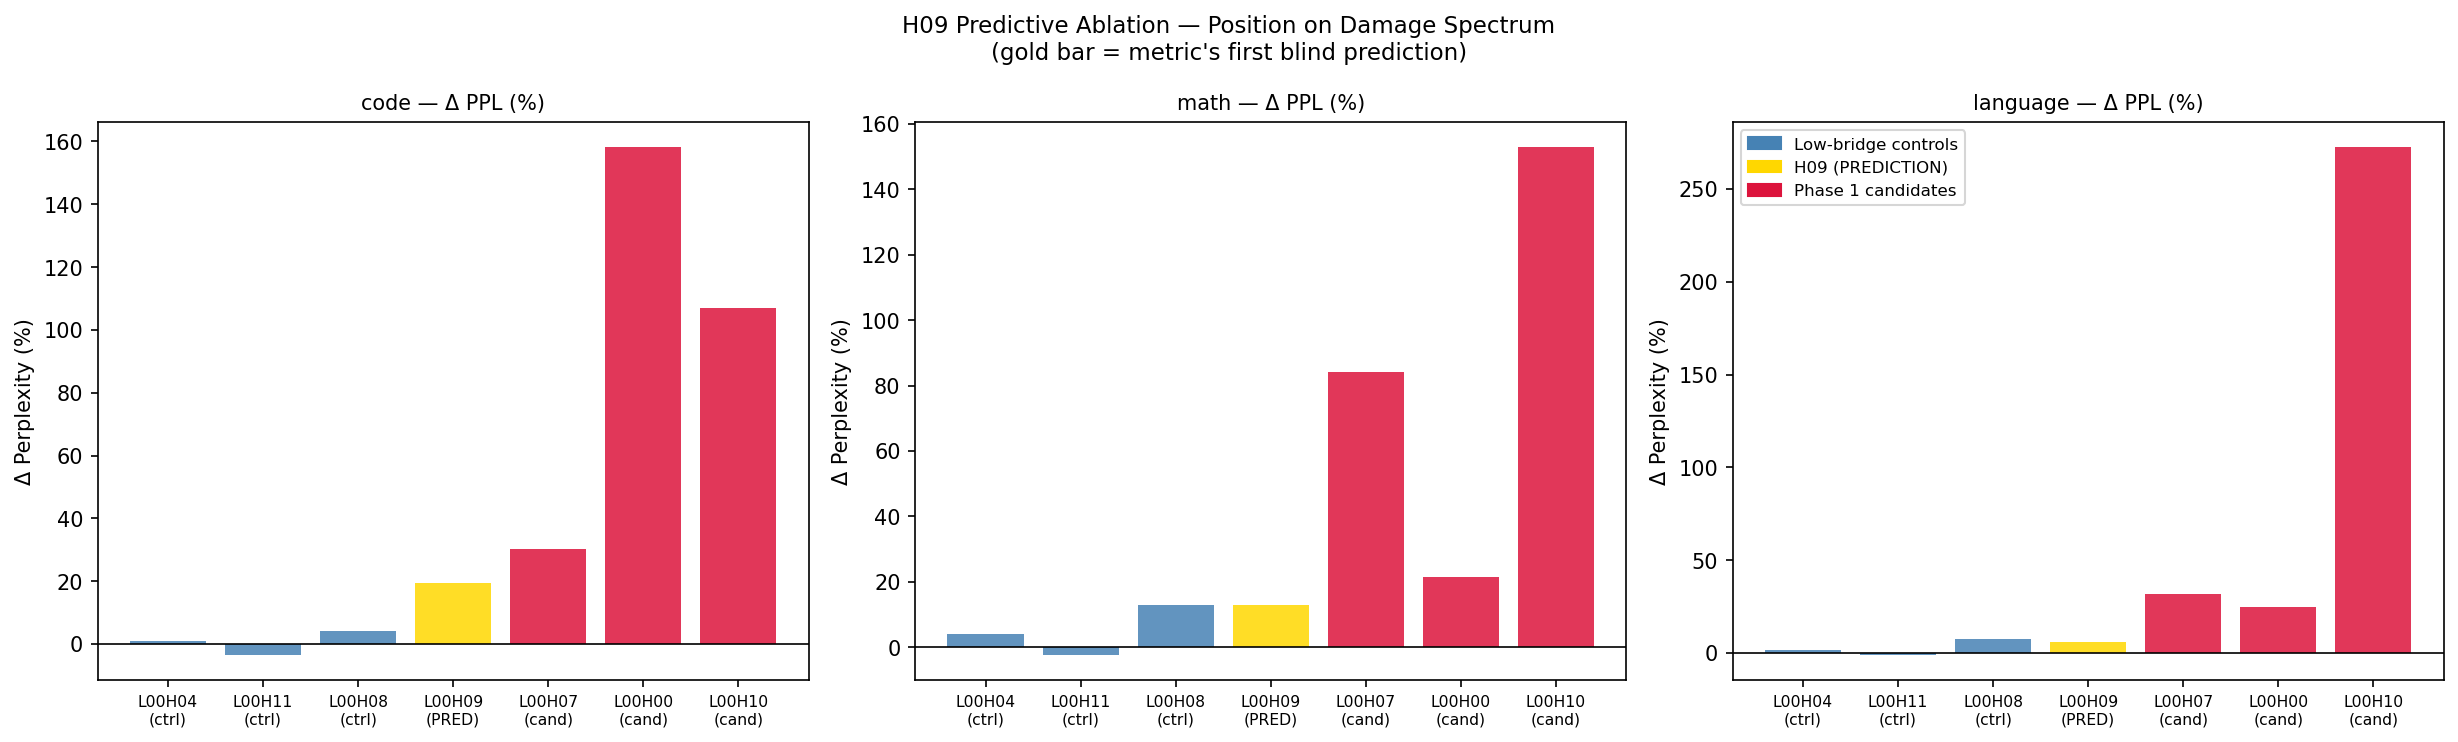
\includegraphics[width=\linewidth]{phase2_h09_prediction.png}
    \caption{%
        \textbf{Bridge score as a prospective predictor.}
        All Layer-0 heads of GPT-2 Small ordered by bridge score.
        \textit{Blue}: low-bridge controls.
        \textit{Gold}: L00H09, the first head tested \emph{after} bridge
        scores were recorded.
        \textit{Red}: Phase~1 candidates.
        L00H09 lands between controls and candidates, exactly as its
        intermediate bridge score predicts.
    \label{fig:prediction}}
\end{figure}

Head L00H09 ($C=13.70$) was identified during the Layer-0 scan but fell
below the Phase~0 threshold.
We ablated L00H09 with no prior knowledge of its damage profile.
Result: $+19.5\%$ (code), $+12.8\%$ (math), $+6.0\%$ (language); mean
$12.8\%$.
This places L00H09 between the low-bridge controls ($2.7\%$ mean) and the
nearest candidate L00H07 ($48.8\%$ mean), precisely consistent with its
intermediate bridge score ($C=13.70$ vs.\ $C=15.56$ for H07;
Figure~\ref{fig:prediction}).
The bridge score generated a correct ordinal prediction about an unseen
head's causal importance before any intervention was conducted.

\paragraph{GPT-2 Medium replication.}
Running Phase~0 on GPT-2 Medium (384 heads across 24 layers) yields
bridge candidates in Layer~2 rather than Layer~0.
This demonstrates that bridge-ness is a \emph{functional}, not positional,
property: it emerges wherever training dynamics create foundational routing
structures used by many subsequent computations.
The main candidate L02H12 ($C_{\text{mix}}=11.40$; $C_{\text{code}}=14.93$)
is the head with the highest predicted causal importance in its layer.
Ordinal ablation confirms this placement.
The separately identified head L02H02 also occupies its predicted ordinal
position relative to low-bridge Layer-2 controls.
In GPT-2 Medium, individual bridge-head ablations cause moderate perplexity
increases (2--9\%), while collective ablation of all candidates causes
33--83\%, consistent with greater functional redundancy at larger scale.

\subsection{Phase 3 and 4: Mechanistic Analysis}
\label{sec:mechanism}

\subsubsection{Downstream Amplification}

\begin{figure}[t]
    \centering
    \begin{subfigure}[t]{0.48\linewidth}
        \centering
        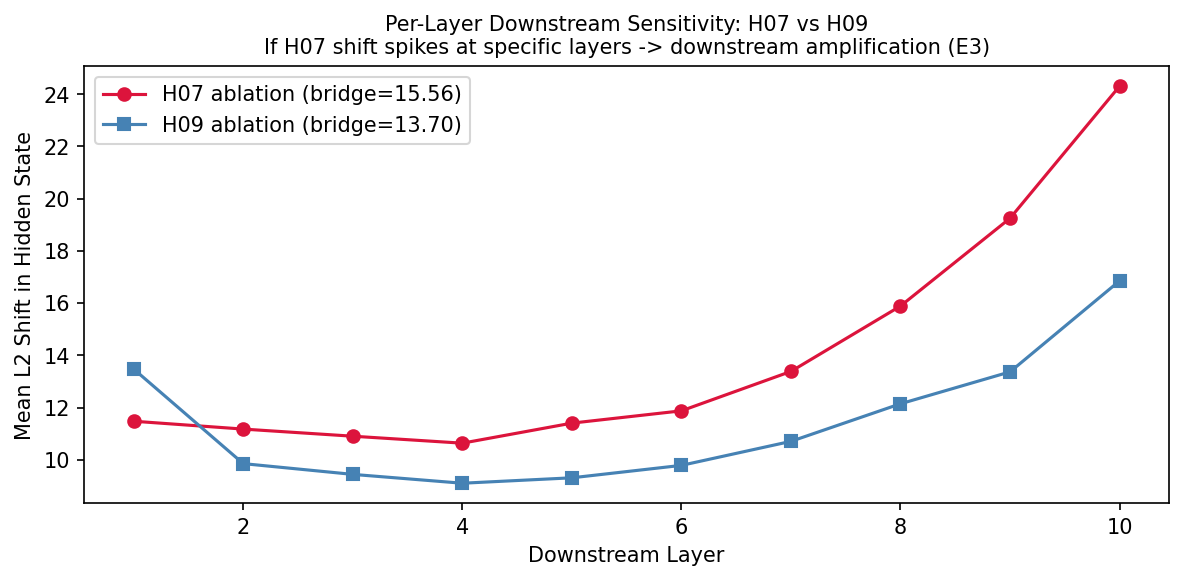
\includegraphics[width=\linewidth]{small_phase3b_downstream_layers.png}
        \caption{GPT-2 Small (Layer-0 heads)}
        \label{fig:amp_small}
    \end{subfigure}
    \hfill
    \begin{subfigure}[t]{0.48\linewidth}
        \centering
        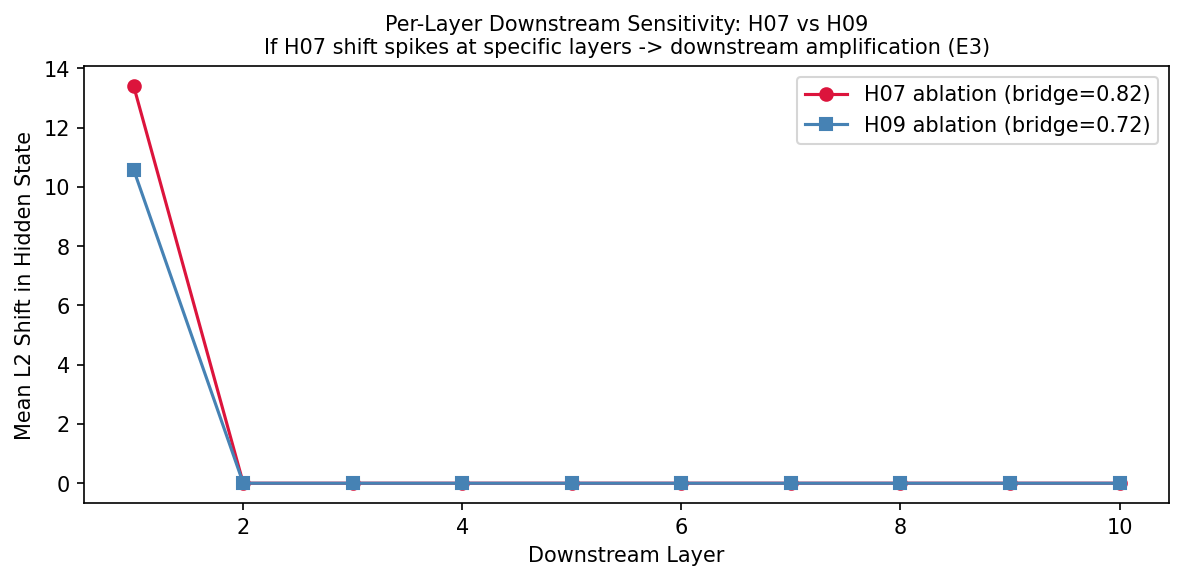
\includegraphics[width=\linewidth]{medium_phase3b_downstream_layers.png}
        \caption{GPT-2 Medium (Layer-2 heads)}
        \label{fig:amp_medium}
    \end{subfigure}
    \caption{%
        \textbf{Per-layer downstream perturbation profiles.}
        Mean L2 shift of the residual stream at each downstream layer
        after ablating H07 (red) and H09 (blue).
        \textbf{(a)} GPT-2 Small: perturbation grows from
        $\approx\!12$ at Layer~1 to $\approx\!24$ at Layer~10 for H07
        (amplification regime).
        \textbf{(b)} GPT-2 Medium (Layer-2 heads with similar bridge
        scores but different function): perturbation collapses within
        two layers (absorption regime).
        These are qualitatively distinct dynamical behaviours, not
        merely a scale difference.
    \label{fig:downstream}}
\end{figure}

Figure~\ref{fig:downstream} shows the downstream perturbation profile
for tested head pairs.
In GPT-2 Small (Figure~\ref{fig:amp_small}), ablating L00H07 produces a
residual-stream shift of $\approx 11.5$ at Layer~1 that grows monotonically
to $\approx 24.3$ at Layer~10 (amplification factor $\approx 2.1\times$).
L00H09 follows the same qualitative trajectory at lower magnitude.
By contrast, ablating Layer-2 heads with similar bridge scores in
GPT-2 Medium (Figure~\ref{fig:amp_medium}) produces a large shift at
Layer~3 that collapses to near zero by Layer~5, an absorption regime in
which subsequent layers correct rather than compound the perturbation.
The GPT-2 Small result is not simply ``more disruption'': it is a
different dynamical regime.

\subsubsection{Amplification Correlates with Bridge Score}

\begin{figure}[t]
    \centering
    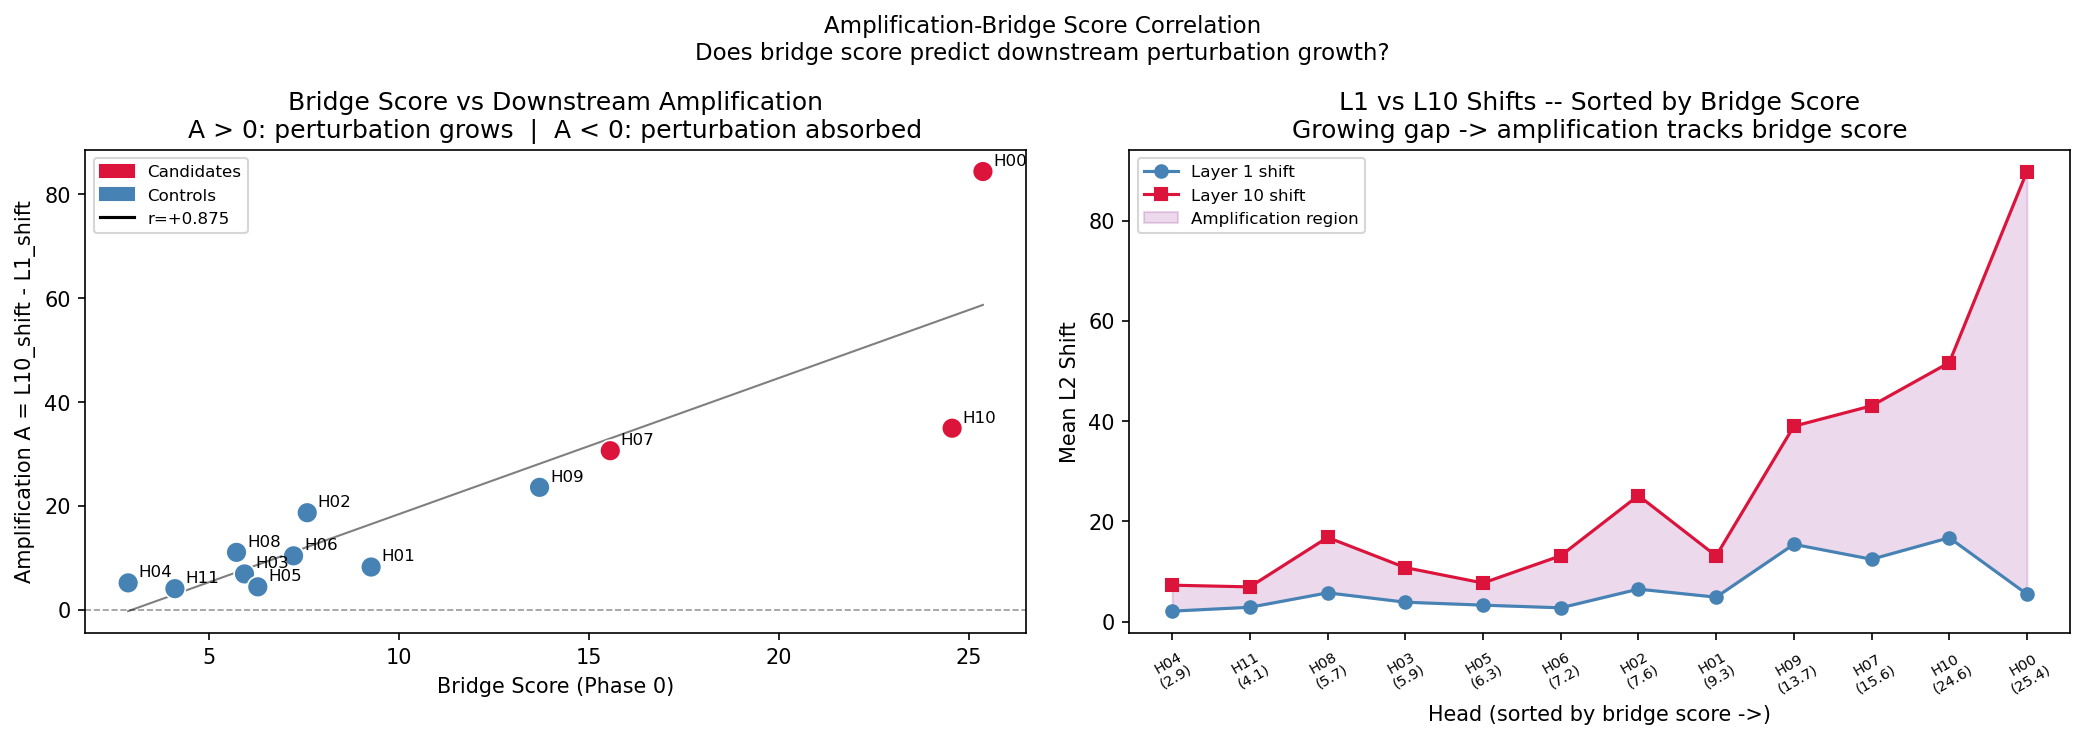
\includegraphics[width=\linewidth]{phase4b_amplification.png}
    \caption{%
        \textbf{Bridge score vs.\ amplification $A(u)$ (GPT-2 Small).}
        \textit{Left:} Scatter of $C(u)$ vs.\ $A(u)$ for all 12
        Layer-0 heads with linear fit ($r=+0.875$, $n=12$, $p<0.001$;
        95\% bootstrap CI $[0.80,\, 0.98]$).
        The correlation is not driven by any single head: removing
        L00H00 yields $r=+0.919$.
        \textit{Right:} Layer-1 and Layer-10 shifts sorted by bridge score;
        the growing pink region shows amplification increasing with bridge
        score.
    \label{fig:amp_corr}}
\end{figure}

Figure~\ref{fig:amp_corr} plots $C(u)$ against $A(u)$ (Eq.~\ref{eq:amp})
for all 12 Layer-0 heads of GPT-2 Small.
The Pearson correlation is $r=+0.875$ ($n=12$, $p<0.001$, two-tailed;
95\% bootstrap CI $[0.80,\, 0.98]$, $10{,}000$ resamples).
This relationship is not driven by any single head: leave-one-out
analysis shows that removing any head keeps $r \geq +0.87$, and
removing L00H00 actually \emph{increases} $r$ to $+0.919$ ($p<0.001$),
indicating the correlation is robust rather than outlier-dependent.
The correlation replicates in GPT-2 Medium Layer-2 heads: $r=+0.715$
($n=16$, $p<0.002$; 95\% bootstrap CI $[0.40,\, 0.90]$).
We interpret this as evidence consistent with the hypothesis that bridge
score preferentially identifies attention heads whose perturbations are
associated with greater downstream amplification, consistent with routing
signals whose effects compound through successive transformer layers
rather than being absorbed.

\subsubsection{Domain Specialisation}
\label{sec:domain_results}

\begin{figure}[t]
    \centering
    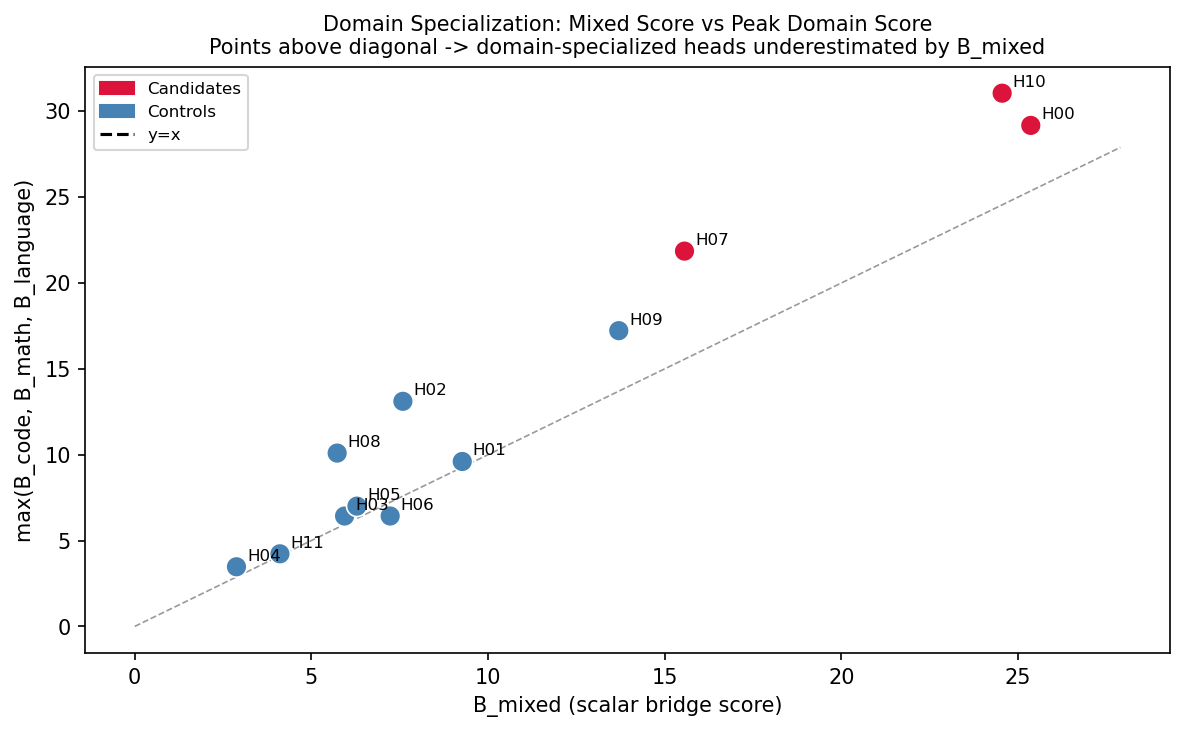
\includegraphics[width=\linewidth]{phase4a_specialization.png}
    \caption{%
        \textbf{Scalar compression of domain specialisation.}
        Mixed bridge score ($C_{\text{mix}}$, x-axis) vs.\ peak domain
        score ($\max_d C_d$, y-axis) for all 12 Layer-0 heads.
        Points above the dashed diagonal are domain-specialised heads
        whose importance is underestimated by the scalar metric.
        All three bridge candidates (red) lie above the diagonal.
    \label{fig:specialization}}
\end{figure}

Figure~\ref{fig:specialization} plots $C_{\text{mix}}(u)$ against
$\max_d C_d(u)$ for all 12 Layer-0 heads.
All three bridge candidates lie above the diagonal: the scalar metric
underestimates their peak domain-specific importance.
H07 is the most specialised: $C_{\text{math}}=21.86$ vs.\
$C_{\text{code}}=14.20$ (ratio $1.54\times$), consistent with its Phase~1
domain damage profile (math $+84\%$ vs.\ code $+30\%$).
H00 is code-elevated: $C_{\text{code}}=29.18$ vs.\
$C_{\text{math}}=26.30$.
H10 shows broadly elevated domain scores
($C_{\text{code}}=26.3$, $C_{\text{math}}=31.1$, $C_{\text{lang}}=28.8$),
consistent with a broadly important routing role.
We note, however, that H10's disproportionately large language damage
($+272\%$) is not fully explained by its language bridge score, which is
not the highest of the three domain scores.
This remains an open question.
Possible explanations include higher-order circuit interactions, nonlinear
amplification specific to the language pathway, or interactions with
attention heads in later layers that we have not yet characterised.
We deliberately refrain from forcing an interpretation and flag this
discrepancy as the most important unresolved finding of the current work.

\subsubsection{Attention Structure}

\begin{figure}[t]
    \centering
    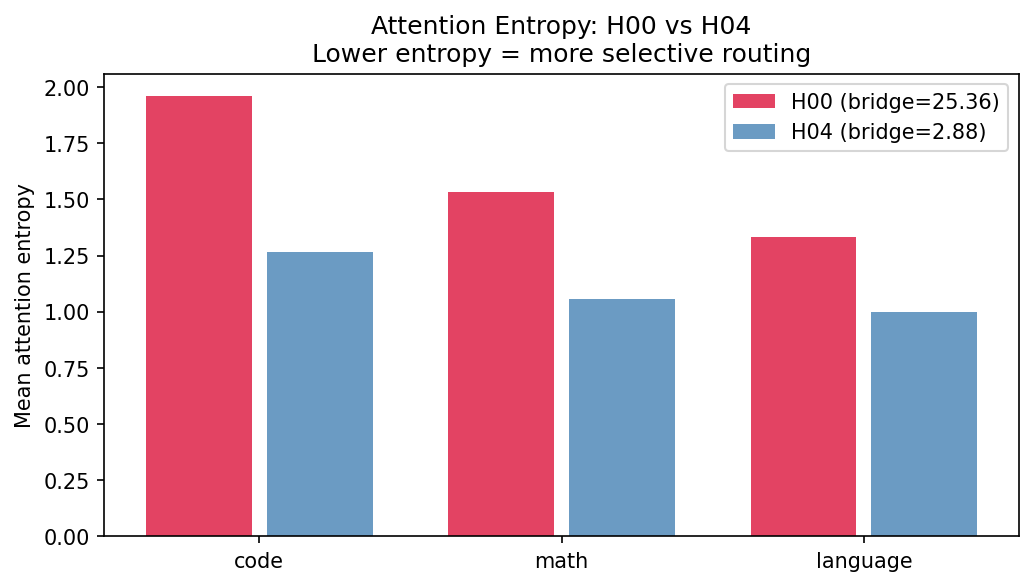
\includegraphics[width=\linewidth]{small_phase3_entropy.png}
    \caption{%
        \textbf{Attention entropy: bridge head vs.\ low-bridge control.}
        L00H00 (bridge, red) exhibits \emph{higher} entropy than L00H04
        (control, blue) in code and math domains.
        Attention heatmaps confirm L00H04 follows a near-diagonal
        (previous-token) pattern while L00H00 shows off-diagonal,
        long-range structure varying with domain.
    \label{fig:entropy}}
\end{figure}

Figure~\ref{fig:entropy} shows mean attention entropy for L00H00 vs.\
L00H04.
Contrary to the intuition that bridge heads are more \emph{focused},
L00H00 exhibits \emph{higher} entropy in code ($1.97$ vs.\ $1.26$) and
math ($1.54$ vs.\ $1.06$) domains.
Attention heatmaps reveal that L00H04 follows near-diagonal (local,
previous-token) attention patterns, while L00H00 shows off-diagonal,
long-range structure that varies with domain.
We interpret this as consistent with a head integrating information from
distant positions to construct routing signals that downstream layers
build upon a structurally diffuse role that appears low-importance by
weight magnitude but is foundational for downstream computation.

\paragraph{Per-token loss maps.}
Ablating L00H07 produces concentrated per-token loss increases on
mathematical function words in math text (\textit{vert}: $+4.3$,
\textit{if}: $+2.0$, \textit{and}: $+2.0$) and on narrative connectors
in language text.
L00H09, with lower bridge score, produces the same token-level pattern
at approximately $10\times$ lower magnitude, a quantitative difference,
not a qualitative one, consistent with the amplification picture.

% ═════════════════════════════════════════════════════════════════════════════
\section{Discussion}
\label{sec:discussion}

\paragraph{What bridge score appears to be measuring.}
The evidence across five experimental phases is consistent with a
coherent account.
Bridge score identifies heads that:
(i) are orthogonal to weight magnitude;
(ii) cause disproportionate causal damage when ablated;
(iii) are not adequately explained by layer position or attention-sink
mechanics alone;
(iv) can be prospectively ranked before any ablation;
(v) exhibit downstream perturbation amplification quantitatively
associated with their bridge score.
The most parsimonious interpretation consistent with the current data
is that these heads inject routing signals into the residual stream that
subsequent layers \emph{use} rather than correct, so their removal does
not merely degrade one layer's computation but corrupts the substrate
for everything that follows.

\paragraph{Bridge-head position is model-specific.}
GPT-2 Small concentrates its bridge heads in Layer~0; GPT-2 Medium
distributes its bridge candidates to Layer~2 and beyond.
Bridge-ness appears to be a functional property that emerges wherever
training dynamics require a layer to construct foundational routing signals
used by many subsequent computations.

\paragraph{Implications for pruning.}
Magnitude-based pruning will systematically target invisible bridge heads
while retaining redundant high-weight heads.
A practical improvement is to add bridge score as a filter: prune only
heads with low weight magnitude \emph{and} low bridge score.
This requires one forward-pass scan per layer, a small additional cost
relative to a full model evaluation.

\paragraph{Relationship to the circuits literature.}
The circuits framework \citep{elhage2021mathematical,olsson2022induction}
identifies important components through activation patching and functional
circuit analysis.
Bridge score offers a cheaper discovery procedure that flags heads with
consequential dynamics without requiring identification of specific
computational algorithms.
Per-token loss maps and domain-conditional scores can then be applied to
understand \emph{what} a bridge head computes once it has been discovered.

\subsection{Threats to Validity}
\label{sec:threats}

\paragraph{Internal validity.}
All ablations use hook-based zeroing of the $c_{\text{proj}}$ input slice.
We verified that this produces identical perplexity to permanent weight
zeroing for all tested heads, but other ablation strategies
(e.g., mean-ablation or noise injection) could in principle yield
different damage rankings.
The probe set ($|\mathcal{P}|=15$ texts per domain) was fixed before
all ablation experiments, but was hand-selected rather than sampled from
a formal distribution; different probe sets might shift individual bridge
scores.

\paragraph{External validity.}
All experiments are conducted on two GPT-2 variants (117M and 345M
parameters).
Whether invisible bridges exist at billion-parameter scale, in
non-autoregressive architectures, or in languages other than English
remains untested.
The probe corpus is exclusively English-language text.

\paragraph{Statistical validity.}
Correlation analyses are conducted over $n=12$ (Small) and $n=16$ (Medium)
heads.
Bootstrap confidence intervals partially address small-sample uncertainty
(95\% CI $[0.80,\,0.98]$ and $[0.40,\,0.90]$ respectively), but the
point estimates should be interpreted cautiously given the limited
sample sizes.
Leave-one-out analysis confirms that no single head drives the
correlation in GPT-2 Small ($r \geq +0.87$ for all deletions).

\paragraph{Construct validity.}
Bridge score measures downstream representation sensitivity---the degree
to which ablating a head shifts subsequent residual-stream states.
This is a necessary but not sufficient condition for functional importance:
a head could shift representations without affecting task performance.
The causal ablation experiments (Phase~1) provide the complementary
evidence that the shifts detected by bridge score do correspond to
performance degradation, but the metric itself should be understood as
measuring \emph{sensitivity} rather than \emph{importance} directly.
Perplexity is the primary performance metric; task-specific capability
collapse is characterised through domain damage profiles but not
formally benchmarked on standard NLP evaluations.
The mechanism for H10's disproportionately large language ablation damage
($+272\%$) remains unexplained and represents the most important
unresolved finding of the current work.

% ═════════════════════════════════════════════════════════════════════════════
\section{Conclusion}
\label{sec:conclusion}

We introduced downstream representation sensitivity: a gradient-free,
probe-based metric that identifies attention heads whose ablation causes
catastrophically disproportionate damage despite near-minimum weight
magnitude.
These \emph{invisible bridges} survive five successive falsification
attempts: metric independence, Layer-0 control ablations, attention-sink
variance tests, prospective ordinal prediction, and cross-model replication.
Downstream perturbation amplification correlates with bridge score
in both GPT-2 Small ($r=+0.875$, 95\% CI $[0.80, 0.98]$) and
GPT-2 Medium ($r=+0.715$, 95\% CI $[0.40, 0.90]$), providing
mechanistic evidence consistent with routing signals that compound rather
than attenuate through successive transformer layers.

Our central finding, that magnitude-based importance rankings are
\emph{inverted} for the most structurally critical attention heads,
challenges a foundational assumption of the neural-network pruning
literature and motivates incorporating structural, relational importance
signals into pruning pipelines.

% ── Bibliography ─────────────────────────────────────────────────────────────
\bibliographystyle{plainnat}
\bibliography{references}

% ═════════════════════════════════════════════════════════════════════════════
\appendix

\section{Experimental Details}
\label{app:details}

\paragraph{Figure files.}
Place the following files in the same Overleaf project directory as this
\texttt{.tex} file (or a \texttt{figures/} subdirectory, updating paths
accordingly):
\begin{itemize}[topsep=2pt,itemsep=1pt,noitemsep]
    \item \texttt{phase0\_scatter.png}
    \item \texttt{phase1\_5\_comparison.png}
    \item \texttt{phase2\_h09\_prediction.png}
    \item \texttt{small\_phase3b\_downstream\_layers.png}
    \item \texttt{medium\_phase3b\_downstream\_layers.png}
    \item \texttt{phase4b\_amplification.png}
    \item \texttt{phase4a\_specialization.png}
    \item \texttt{small\_phase3\_entropy.png}
\end{itemize}

\paragraph{Ablation implementation.}
All ablations use \texttt{torch.nn.Module.register\_forward\_pre\_hook}
applied to the \texttt{attn.c\_proj} submodule at the target layer.
The hook zeroes the slice $x_{[:,:,s:e]}$ of the pre-projection input,
where $s=k\,d_h$, $e=(k+1)\,d_h$, $d_h=d/H$.
We verified that hook-based zeroing produces identical perplexity values
to permanent weight zeroing (zeroing rows $[s:e,:]$ of the c\_proj
weight matrix) for all tested heads.

\paragraph{Perplexity computation.}
Perplexity is computed as
$\exp\!\bigl(\frac{1}{N}\sum_{i=1}^{N}\mathcal{L}_i\bigr)$
where $\mathcal{L}_i$ is the per-token cross-entropy loss from
\texttt{GPT2LMHeadModel} with \texttt{labels = input\_ids}.
Texts are truncated to 128 tokens.

\section{Complete Experimental Record}
\label{app:tables}

\begin{table}[h]
\centering
\caption{Summary of all experimental phases.}
\label{tab:summary}
\small
\begin{tabularx}{\linewidth}{lXl}
\toprule
\textbf{Phase} & \textbf{Key Result} & \textbf{Interpretation} \\
\midrule
0         & $r(\text{Bridge},\,\text{Wanda})\approx 0$ (all domains)
          & Independent signals \\
1         & Mean damage ratio A/B $= 213\times$
          & Bridges are causally critical \\
1.5       & Low-bridge L0 controls: $2.7\%$ damage
          & Layer position insufficient \\
1.5       & Bridge head attention variance $\sigma>0.09$
          & Sink behavior insufficient \\
2 (Small) & H09 damage $12.8\%$; ordinal position correct
          & Prospective prediction \\
2 (Med.)  & L02H02, L02H12 ordinal positions correct
          & Cross-model prediction \\
3 (Small) & H07: L1 $\to$ L10 shift grows $11.5\to24.3$
          & Consistent with amplification \\
3 (Med.)  & Same heads: L1 shift collapses to $\approx0$
          & Absorption in Medium \\
3b        & H07 math $93\%$ vs.\ H09 math $13\%$
          & Domain specialisation \\
4a        & All candidates above B\_mix diagonal
          & Scalar compresses specialisation \\
4b (Small)& $r(\text{Bridge},\,A)=+0.875$, CI $[0.80, 0.98]$
          & Mechanistic evidence (Small) \\
4b (Med.) & $r(\text{Bridge},\,A)=+0.715$, CI $[0.40, 0.90]$
          & Mechanistic evidence (Medium) \\
\bottomrule
\end{tabularx}
\end{table}

\end{document}